\chapter{Introduction}
\label{ch:introduction}
% Mixed Reality-Driving Simulator developed using Unity 3D-Engine 
Augmented reality has not only changed the perception of the world for the ordinary user but it has also allowed researchers to conduct studies which have not been possible before. The chair of Human Machine Communication is currently developing a mixed reality driving simulator using Unity Engine in a 3D CAVE. It can be utilised to facilitate studies regarding reaction of the driver in different situations on the road and development of better Head-Up Displays.

Currently, the 3D models which simulate the street network are generated using ESRI CityEngine and unfortunately, they are not based on real data. Moreover, a semantical description of the underlaying street network, as well as any properties of its segment are not present. Street information based on real data exported from open source projects such as OpenStreetMap would improve the quality of the generated models. This would allow the simulation of real scenes and furthermore facilitate the research of the human-machine interaction. Additionally, a semantical description of the street network would allow the simulation of autonomous vehicles and fully simulation of traffic management system. 
 
\section{Goals of the Project}
\label{sec:goals}
The main goal of this Interdisciplinary Project is to derive semantical description of the road network, generated using OpenStreetMap data in CityEngine and SUMO. Moreover, the generated 3D scene of a city model has to be synchronised with the aforementioned description. Additionally, the export document has to contain all details about the lanes which compose all corresponding road segments and their properties, as well as the coordinates of buildings and parkings which can be found in the generated scene. The export must be accomplished in a widely compatible format which has proven suitable for these purposes, as well. Finally, the road network description has to be imported in the MMK Driving Simulator in order to build a navigation system for the traffic participants using the already generated connectivity information by SUMO.

\section{Outline}
\label{sec:outline}
The remainder of this report is organised as follows: Chapter \ref{ch:background} provides background information about the essential tools which are used to improve the current functionalities of the MMK Driving Simulator. Later, in Chapter \ref{ch:descriptionOfRoadSystems}, we describe thoroughly our approach to derive a semantical description of the road system generated in CityEngine from OpenStreetMap data. Moreover, we discuss how additional road information can be derived from SUMO simulation files about the same road system. Afterwards, Chapter \ref{ch:gps} presents how we can furthermore utilise the SUMO-generated road connectivity information to construct a navigation system. Finally, Chapter \ref{ch:conclusion} makes a summary of the achieved goals and discusses possibilities for future improvements of the project.  

%\begin{figure}[htb]
%	\centering
%	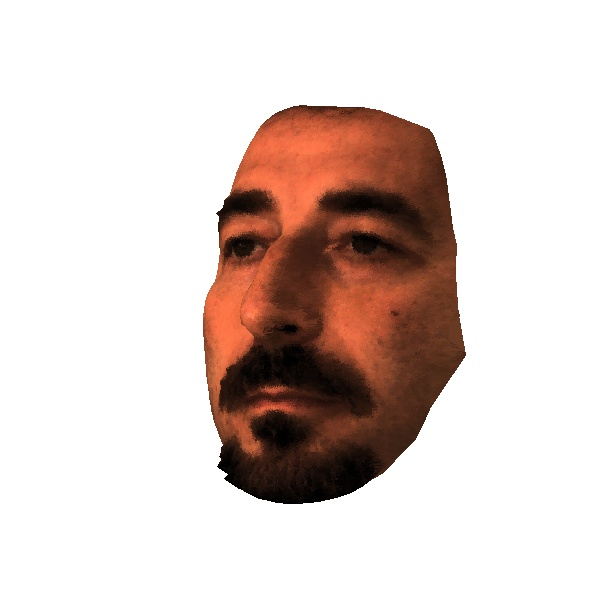
\includegraphics[width=0.35\linewidth]{figures/figure}
%	\caption{Some sample figure.}
%	\label{fig:sample}
%\end{figure}
